\documentclass[11pt]{article}

    \usepackage[breakable]{tcolorbox}
    \usepackage{parskip} % Stop auto-indenting (to mimic markdown behaviour)
    
    \usepackage{iftex}
    \ifPDFTeX
    	\usepackage[T1]{fontenc}
    	\usepackage{mathpazo}
    \else
    	\usepackage{fontspec}
    \fi

    % Basic figure setup, for now with no caption control since it's done
    % automatically by Pandoc (which extracts ![](path) syntax from Markdown).
    \usepackage{graphicx}
    % Maintain compatibility with old templates. Remove in nbconvert 6.0
    \let\Oldincludegraphics\includegraphics
    % Ensure that by default, figures have no caption (until we provide a
    % proper Figure object with a Caption API and a way to capture that
    % in the conversion process - todo).
    \usepackage{caption}
    \DeclareCaptionFormat{nocaption}{}
    \captionsetup{format=nocaption,aboveskip=0pt,belowskip=0pt}

    \usepackage{float}
    \floatplacement{figure}{H} % forces figures to be placed at the correct location
    \usepackage{xcolor} % Allow colors to be defined
    \usepackage{enumerate} % Needed for markdown enumerations to work
    \usepackage{geometry} % Used to adjust the document margins
    \usepackage{amsmath} % Equations
    \usepackage{amssymb} % Equations
    \usepackage{textcomp} % defines textquotesingle
    % Hack from http://tex.stackexchange.com/a/47451/13684:
    \AtBeginDocument{%
        \def\PYZsq{\textquotesingle}% Upright quotes in Pygmentized code
    }
    \usepackage{upquote} % Upright quotes for verbatim code
    \usepackage{eurosym} % defines \euro
    \usepackage[mathletters]{ucs} % Extended unicode (utf-8) support
    \usepackage{fancyvrb} % verbatim replacement that allows latex
    \usepackage{grffile} % extends the file name processing of package graphics 
                         % to support a larger range
    \makeatletter % fix for old versions of grffile with XeLaTeX
    \@ifpackagelater{grffile}{2019/11/01}
    {
      % Do nothing on new versions
    }
    {
      \def\Gread@@xetex#1{%
        \IfFileExists{"\Gin@base".bb}%
        {\Gread@eps{\Gin@base.bb}}%
        {\Gread@@xetex@aux#1}%
      }
    }
    \makeatother
    \usepackage[Export]{adjustbox} % Used to constrain images to a maximum size
    \adjustboxset{max size={0.9\linewidth}{0.9\paperheight}}

    % The hyperref package gives us a pdf with properly built
    % internal navigation ('pdf bookmarks' for the table of contents,
    % internal cross-reference links, web links for URLs, etc.)
    \usepackage{hyperref}
    % The default LaTeX title has an obnoxious amount of whitespace. By default,
    % titling removes some of it. It also provides customization options.
    \usepackage{titling}
    \usepackage{longtable} % longtable support required by pandoc >1.10
    \usepackage{booktabs}  % table support for pandoc > 1.12.2
    \usepackage[inline]{enumitem} % IRkernel/repr support (it uses the enumerate* environment)
    \usepackage[normalem]{ulem} % ulem is needed to support strikethroughs (\sout)
                                % normalem makes italics be italics, not underlines
    \usepackage{mathrsfs}
    

    
    % Colors for the hyperref package
    \definecolor{urlcolor}{rgb}{0,.145,.698}
    \definecolor{linkcolor}{rgb}{.71,0.21,0.01}
    \definecolor{citecolor}{rgb}{.12,.54,.11}

    % ANSI colors
    \definecolor{ansi-black}{HTML}{3E424D}
    \definecolor{ansi-black-intense}{HTML}{282C36}
    \definecolor{ansi-red}{HTML}{E75C58}
    \definecolor{ansi-red-intense}{HTML}{B22B31}
    \definecolor{ansi-green}{HTML}{00A250}
    \definecolor{ansi-green-intense}{HTML}{007427}
    \definecolor{ansi-yellow}{HTML}{DDB62B}
    \definecolor{ansi-yellow-intense}{HTML}{B27D12}
    \definecolor{ansi-blue}{HTML}{208FFB}
    \definecolor{ansi-blue-intense}{HTML}{0065CA}
    \definecolor{ansi-magenta}{HTML}{D160C4}
    \definecolor{ansi-magenta-intense}{HTML}{A03196}
    \definecolor{ansi-cyan}{HTML}{60C6C8}
    \definecolor{ansi-cyan-intense}{HTML}{258F8F}
    \definecolor{ansi-white}{HTML}{C5C1B4}
    \definecolor{ansi-white-intense}{HTML}{A1A6B2}
    \definecolor{ansi-default-inverse-fg}{HTML}{FFFFFF}
    \definecolor{ansi-default-inverse-bg}{HTML}{000000}

    % common color for the border for error outputs.
    \definecolor{outerrorbackground}{HTML}{FFDFDF}

    % commands and environments needed by pandoc snippets
    % extracted from the output of `pandoc -s`
    \providecommand{\tightlist}{%
      \setlength{\itemsep}{0pt}\setlength{\parskip}{0pt}}
    \DefineVerbatimEnvironment{Highlighting}{Verbatim}{commandchars=\\\{\}}
    % Add ',fontsize=\small' for more characters per line
    \newenvironment{Shaded}{}{}
    \newcommand{\KeywordTok}[1]{\textcolor[rgb]{0.00,0.44,0.13}{\textbf{{#1}}}}
    \newcommand{\DataTypeTok}[1]{\textcolor[rgb]{0.56,0.13,0.00}{{#1}}}
    \newcommand{\DecValTok}[1]{\textcolor[rgb]{0.25,0.63,0.44}{{#1}}}
    \newcommand{\BaseNTok}[1]{\textcolor[rgb]{0.25,0.63,0.44}{{#1}}}
    \newcommand{\FloatTok}[1]{\textcolor[rgb]{0.25,0.63,0.44}{{#1}}}
    \newcommand{\CharTok}[1]{\textcolor[rgb]{0.25,0.44,0.63}{{#1}}}
    \newcommand{\StringTok}[1]{\textcolor[rgb]{0.25,0.44,0.63}{{#1}}}
    \newcommand{\CommentTok}[1]{\textcolor[rgb]{0.38,0.63,0.69}{\textit{{#1}}}}
    \newcommand{\OtherTok}[1]{\textcolor[rgb]{0.00,0.44,0.13}{{#1}}}
    \newcommand{\AlertTok}[1]{\textcolor[rgb]{1.00,0.00,0.00}{\textbf{{#1}}}}
    \newcommand{\FunctionTok}[1]{\textcolor[rgb]{0.02,0.16,0.49}{{#1}}}
    \newcommand{\RegionMarkerTok}[1]{{#1}}
    \newcommand{\ErrorTok}[1]{\textcolor[rgb]{1.00,0.00,0.00}{\textbf{{#1}}}}
    \newcommand{\NormalTok}[1]{{#1}}
    
    % Additional commands for more recent versions of Pandoc
    \newcommand{\ConstantTok}[1]{\textcolor[rgb]{0.53,0.00,0.00}{{#1}}}
    \newcommand{\SpecialCharTok}[1]{\textcolor[rgb]{0.25,0.44,0.63}{{#1}}}
    \newcommand{\VerbatimStringTok}[1]{\textcolor[rgb]{0.25,0.44,0.63}{{#1}}}
    \newcommand{\SpecialStringTok}[1]{\textcolor[rgb]{0.73,0.40,0.53}{{#1}}}
    \newcommand{\ImportTok}[1]{{#1}}
    \newcommand{\DocumentationTok}[1]{\textcolor[rgb]{0.73,0.13,0.13}{\textit{{#1}}}}
    \newcommand{\AnnotationTok}[1]{\textcolor[rgb]{0.38,0.63,0.69}{\textbf{\textit{{#1}}}}}
    \newcommand{\CommentVarTok}[1]{\textcolor[rgb]{0.38,0.63,0.69}{\textbf{\textit{{#1}}}}}
    \newcommand{\VariableTok}[1]{\textcolor[rgb]{0.10,0.09,0.49}{{#1}}}
    \newcommand{\ControlFlowTok}[1]{\textcolor[rgb]{0.00,0.44,0.13}{\textbf{{#1}}}}
    \newcommand{\OperatorTok}[1]{\textcolor[rgb]{0.40,0.40,0.40}{{#1}}}
    \newcommand{\BuiltInTok}[1]{{#1}}
    \newcommand{\ExtensionTok}[1]{{#1}}
    \newcommand{\PreprocessorTok}[1]{\textcolor[rgb]{0.74,0.48,0.00}{{#1}}}
    \newcommand{\AttributeTok}[1]{\textcolor[rgb]{0.49,0.56,0.16}{{#1}}}
    \newcommand{\InformationTok}[1]{\textcolor[rgb]{0.38,0.63,0.69}{\textbf{\textit{{#1}}}}}
    \newcommand{\WarningTok}[1]{\textcolor[rgb]{0.38,0.63,0.69}{\textbf{\textit{{#1}}}}}
    
    
    % Define a nice break command that doesn't care if a line doesn't already
    % exist.
    \def\br{\hspace*{\fill} \\* }
    % Math Jax compatibility definitions
    \def\gt{>}
    \def\lt{<}
    \let\Oldtex\TeX
    \let\Oldlatex\LaTeX
    \renewcommand{\TeX}{\textrm{\Oldtex}}
    \renewcommand{\LaTeX}{\textrm{\Oldlatex}}
    % Document parameters
    % Document title
    \title{Lecture 2 - Part 1: Introduction to numpy and scipy}
    \date{}
    
    
    
    
% Pygments definitions
\makeatletter
\def\PY@reset{\let\PY@it=\relax \let\PY@bf=\relax%
    \let\PY@ul=\relax \let\PY@tc=\relax%
    \let\PY@bc=\relax \let\PY@ff=\relax}
\def\PY@tok#1{\csname PY@tok@#1\endcsname}
\def\PY@toks#1+{\ifx\relax#1\empty\else%
    \PY@tok{#1}\expandafter\PY@toks\fi}
\def\PY@do#1{\PY@bc{\PY@tc{\PY@ul{%
    \PY@it{\PY@bf{\PY@ff{#1}}}}}}}
\def\PY#1#2{\PY@reset\PY@toks#1+\relax+\PY@do{#2}}

\@namedef{PY@tok@w}{\def\PY@tc##1{\textcolor[rgb]{0.73,0.73,0.73}{##1}}}
\@namedef{PY@tok@c}{\let\PY@it=\textit\def\PY@tc##1{\textcolor[rgb]{0.25,0.50,0.50}{##1}}}
\@namedef{PY@tok@cp}{\def\PY@tc##1{\textcolor[rgb]{0.74,0.48,0.00}{##1}}}
\@namedef{PY@tok@k}{\let\PY@bf=\textbf\def\PY@tc##1{\textcolor[rgb]{0.00,0.50,0.00}{##1}}}
\@namedef{PY@tok@kp}{\def\PY@tc##1{\textcolor[rgb]{0.00,0.50,0.00}{##1}}}
\@namedef{PY@tok@kt}{\def\PY@tc##1{\textcolor[rgb]{0.69,0.00,0.25}{##1}}}
\@namedef{PY@tok@o}{\def\PY@tc##1{\textcolor[rgb]{0.40,0.40,0.40}{##1}}}
\@namedef{PY@tok@ow}{\let\PY@bf=\textbf\def\PY@tc##1{\textcolor[rgb]{0.67,0.13,1.00}{##1}}}
\@namedef{PY@tok@nb}{\def\PY@tc##1{\textcolor[rgb]{0.00,0.50,0.00}{##1}}}
\@namedef{PY@tok@nf}{\def\PY@tc##1{\textcolor[rgb]{0.00,0.00,1.00}{##1}}}
\@namedef{PY@tok@nc}{\let\PY@bf=\textbf\def\PY@tc##1{\textcolor[rgb]{0.00,0.00,1.00}{##1}}}
\@namedef{PY@tok@nn}{\let\PY@bf=\textbf\def\PY@tc##1{\textcolor[rgb]{0.00,0.00,1.00}{##1}}}
\@namedef{PY@tok@ne}{\let\PY@bf=\textbf\def\PY@tc##1{\textcolor[rgb]{0.82,0.25,0.23}{##1}}}
\@namedef{PY@tok@nv}{\def\PY@tc##1{\textcolor[rgb]{0.10,0.09,0.49}{##1}}}
\@namedef{PY@tok@no}{\def\PY@tc##1{\textcolor[rgb]{0.53,0.00,0.00}{##1}}}
\@namedef{PY@tok@nl}{\def\PY@tc##1{\textcolor[rgb]{0.63,0.63,0.00}{##1}}}
\@namedef{PY@tok@ni}{\let\PY@bf=\textbf\def\PY@tc##1{\textcolor[rgb]{0.60,0.60,0.60}{##1}}}
\@namedef{PY@tok@na}{\def\PY@tc##1{\textcolor[rgb]{0.49,0.56,0.16}{##1}}}
\@namedef{PY@tok@nt}{\let\PY@bf=\textbf\def\PY@tc##1{\textcolor[rgb]{0.00,0.50,0.00}{##1}}}
\@namedef{PY@tok@nd}{\def\PY@tc##1{\textcolor[rgb]{0.67,0.13,1.00}{##1}}}
\@namedef{PY@tok@s}{\def\PY@tc##1{\textcolor[rgb]{0.73,0.13,0.13}{##1}}}
\@namedef{PY@tok@sd}{\let\PY@it=\textit\def\PY@tc##1{\textcolor[rgb]{0.73,0.13,0.13}{##1}}}
\@namedef{PY@tok@si}{\let\PY@bf=\textbf\def\PY@tc##1{\textcolor[rgb]{0.73,0.40,0.53}{##1}}}
\@namedef{PY@tok@se}{\let\PY@bf=\textbf\def\PY@tc##1{\textcolor[rgb]{0.73,0.40,0.13}{##1}}}
\@namedef{PY@tok@sr}{\def\PY@tc##1{\textcolor[rgb]{0.73,0.40,0.53}{##1}}}
\@namedef{PY@tok@ss}{\def\PY@tc##1{\textcolor[rgb]{0.10,0.09,0.49}{##1}}}
\@namedef{PY@tok@sx}{\def\PY@tc##1{\textcolor[rgb]{0.00,0.50,0.00}{##1}}}
\@namedef{PY@tok@m}{\def\PY@tc##1{\textcolor[rgb]{0.40,0.40,0.40}{##1}}}
\@namedef{PY@tok@gh}{\let\PY@bf=\textbf\def\PY@tc##1{\textcolor[rgb]{0.00,0.00,0.50}{##1}}}
\@namedef{PY@tok@gu}{\let\PY@bf=\textbf\def\PY@tc##1{\textcolor[rgb]{0.50,0.00,0.50}{##1}}}
\@namedef{PY@tok@gd}{\def\PY@tc##1{\textcolor[rgb]{0.63,0.00,0.00}{##1}}}
\@namedef{PY@tok@gi}{\def\PY@tc##1{\textcolor[rgb]{0.00,0.63,0.00}{##1}}}
\@namedef{PY@tok@gr}{\def\PY@tc##1{\textcolor[rgb]{1.00,0.00,0.00}{##1}}}
\@namedef{PY@tok@ge}{\let\PY@it=\textit}
\@namedef{PY@tok@gs}{\let\PY@bf=\textbf}
\@namedef{PY@tok@gp}{\let\PY@bf=\textbf\def\PY@tc##1{\textcolor[rgb]{0.00,0.00,0.50}{##1}}}
\@namedef{PY@tok@go}{\def\PY@tc##1{\textcolor[rgb]{0.53,0.53,0.53}{##1}}}
\@namedef{PY@tok@gt}{\def\PY@tc##1{\textcolor[rgb]{0.00,0.27,0.87}{##1}}}
\@namedef{PY@tok@err}{\def\PY@bc##1{{\setlength{\fboxsep}{\string -\fboxrule}\fcolorbox[rgb]{1.00,0.00,0.00}{1,1,1}{\strut ##1}}}}
\@namedef{PY@tok@kc}{\let\PY@bf=\textbf\def\PY@tc##1{\textcolor[rgb]{0.00,0.50,0.00}{##1}}}
\@namedef{PY@tok@kd}{\let\PY@bf=\textbf\def\PY@tc##1{\textcolor[rgb]{0.00,0.50,0.00}{##1}}}
\@namedef{PY@tok@kn}{\let\PY@bf=\textbf\def\PY@tc##1{\textcolor[rgb]{0.00,0.50,0.00}{##1}}}
\@namedef{PY@tok@kr}{\let\PY@bf=\textbf\def\PY@tc##1{\textcolor[rgb]{0.00,0.50,0.00}{##1}}}
\@namedef{PY@tok@bp}{\def\PY@tc##1{\textcolor[rgb]{0.00,0.50,0.00}{##1}}}
\@namedef{PY@tok@fm}{\def\PY@tc##1{\textcolor[rgb]{0.00,0.00,1.00}{##1}}}
\@namedef{PY@tok@vc}{\def\PY@tc##1{\textcolor[rgb]{0.10,0.09,0.49}{##1}}}
\@namedef{PY@tok@vg}{\def\PY@tc##1{\textcolor[rgb]{0.10,0.09,0.49}{##1}}}
\@namedef{PY@tok@vi}{\def\PY@tc##1{\textcolor[rgb]{0.10,0.09,0.49}{##1}}}
\@namedef{PY@tok@vm}{\def\PY@tc##1{\textcolor[rgb]{0.10,0.09,0.49}{##1}}}
\@namedef{PY@tok@sa}{\def\PY@tc##1{\textcolor[rgb]{0.73,0.13,0.13}{##1}}}
\@namedef{PY@tok@sb}{\def\PY@tc##1{\textcolor[rgb]{0.73,0.13,0.13}{##1}}}
\@namedef{PY@tok@sc}{\def\PY@tc##1{\textcolor[rgb]{0.73,0.13,0.13}{##1}}}
\@namedef{PY@tok@dl}{\def\PY@tc##1{\textcolor[rgb]{0.73,0.13,0.13}{##1}}}
\@namedef{PY@tok@s2}{\def\PY@tc##1{\textcolor[rgb]{0.73,0.13,0.13}{##1}}}
\@namedef{PY@tok@sh}{\def\PY@tc##1{\textcolor[rgb]{0.73,0.13,0.13}{##1}}}
\@namedef{PY@tok@s1}{\def\PY@tc##1{\textcolor[rgb]{0.73,0.13,0.13}{##1}}}
\@namedef{PY@tok@mb}{\def\PY@tc##1{\textcolor[rgb]{0.40,0.40,0.40}{##1}}}
\@namedef{PY@tok@mf}{\def\PY@tc##1{\textcolor[rgb]{0.40,0.40,0.40}{##1}}}
\@namedef{PY@tok@mh}{\def\PY@tc##1{\textcolor[rgb]{0.40,0.40,0.40}{##1}}}
\@namedef{PY@tok@mi}{\def\PY@tc##1{\textcolor[rgb]{0.40,0.40,0.40}{##1}}}
\@namedef{PY@tok@il}{\def\PY@tc##1{\textcolor[rgb]{0.40,0.40,0.40}{##1}}}
\@namedef{PY@tok@mo}{\def\PY@tc##1{\textcolor[rgb]{0.40,0.40,0.40}{##1}}}
\@namedef{PY@tok@ch}{\let\PY@it=\textit\def\PY@tc##1{\textcolor[rgb]{0.25,0.50,0.50}{##1}}}
\@namedef{PY@tok@cm}{\let\PY@it=\textit\def\PY@tc##1{\textcolor[rgb]{0.25,0.50,0.50}{##1}}}
\@namedef{PY@tok@cpf}{\let\PY@it=\textit\def\PY@tc##1{\textcolor[rgb]{0.25,0.50,0.50}{##1}}}
\@namedef{PY@tok@c1}{\let\PY@it=\textit\def\PY@tc##1{\textcolor[rgb]{0.25,0.50,0.50}{##1}}}
\@namedef{PY@tok@cs}{\let\PY@it=\textit\def\PY@tc##1{\textcolor[rgb]{0.25,0.50,0.50}{##1}}}

\def\PYZbs{\char`\\}
\def\PYZus{\char`\_}
\def\PYZob{\char`\{}
\def\PYZcb{\char`\}}
\def\PYZca{\char`\^}
\def\PYZam{\char`\&}
\def\PYZlt{\char`\<}
\def\PYZgt{\char`\>}
\def\PYZsh{\char`\#}
\def\PYZpc{\char`\%}
\def\PYZdl{\char`\$}
\def\PYZhy{\char`\-}
\def\PYZsq{\char`\'}
\def\PYZdq{\char`\"}
\def\PYZti{\char`\~}
% for compatibility with earlier versions
\def\PYZat{@}
\def\PYZlb{[}
\def\PYZrb{]}
\makeatother


    % For linebreaks inside Verbatim environment from package fancyvrb. 
    \makeatletter
        \newbox\Wrappedcontinuationbox 
        \newbox\Wrappedvisiblespacebox 
        \newcommand*\Wrappedvisiblespace {\textcolor{red}{\textvisiblespace}} 
        \newcommand*\Wrappedcontinuationsymbol {\textcolor{red}{\llap{\tiny$\m@th\hookrightarrow$}}} 
        \newcommand*\Wrappedcontinuationindent {3ex } 
        \newcommand*\Wrappedafterbreak {\kern\Wrappedcontinuationindent\copy\Wrappedcontinuationbox} 
        % Take advantage of the already applied Pygments mark-up to insert 
        % potential linebreaks for TeX processing. 
        %        {, <, #, %, $, ' and ": go to next line. 
        %        _, }, ^, &, >, - and ~: stay at end of broken line. 
        % Use of \textquotesingle for straight quote. 
        \newcommand*\Wrappedbreaksatspecials {% 
            \def\PYGZus{\discretionary{\char`\_}{\Wrappedafterbreak}{\char`\_}}% 
            \def\PYGZob{\discretionary{}{\Wrappedafterbreak\char`\{}{\char`\{}}% 
            \def\PYGZcb{\discretionary{\char`\}}{\Wrappedafterbreak}{\char`\}}}% 
            \def\PYGZca{\discretionary{\char`\^}{\Wrappedafterbreak}{\char`\^}}% 
            \def\PYGZam{\discretionary{\char`\&}{\Wrappedafterbreak}{\char`\&}}% 
            \def\PYGZlt{\discretionary{}{\Wrappedafterbreak\char`\<}{\char`\<}}% 
            \def\PYGZgt{\discretionary{\char`\>}{\Wrappedafterbreak}{\char`\>}}% 
            \def\PYGZsh{\discretionary{}{\Wrappedafterbreak\char`\#}{\char`\#}}% 
            \def\PYGZpc{\discretionary{}{\Wrappedafterbreak\char`\%}{\char`\%}}% 
            \def\PYGZdl{\discretionary{}{\Wrappedafterbreak\char`\$}{\char`\$}}% 
            \def\PYGZhy{\discretionary{\char`\-}{\Wrappedafterbreak}{\char`\-}}% 
            \def\PYGZsq{\discretionary{}{\Wrappedafterbreak\textquotesingle}{\textquotesingle}}% 
            \def\PYGZdq{\discretionary{}{\Wrappedafterbreak\char`\"}{\char`\"}}% 
            \def\PYGZti{\discretionary{\char`\~}{\Wrappedafterbreak}{\char`\~}}% 
        } 
        % Some characters . , ; ? ! / are not pygmentized. 
        % This macro makes them "active" and they will insert potential linebreaks 
        \newcommand*\Wrappedbreaksatpunct {% 
            \lccode`\~`\.\lowercase{\def~}{\discretionary{\hbox{\char`\.}}{\Wrappedafterbreak}{\hbox{\char`\.}}}% 
            \lccode`\~`\,\lowercase{\def~}{\discretionary{\hbox{\char`\,}}{\Wrappedafterbreak}{\hbox{\char`\,}}}% 
            \lccode`\~`\;\lowercase{\def~}{\discretionary{\hbox{\char`\;}}{\Wrappedafterbreak}{\hbox{\char`\;}}}% 
            \lccode`\~`\:\lowercase{\def~}{\discretionary{\hbox{\char`\:}}{\Wrappedafterbreak}{\hbox{\char`\:}}}% 
            \lccode`\~`\?\lowercase{\def~}{\discretionary{\hbox{\char`\?}}{\Wrappedafterbreak}{\hbox{\char`\?}}}% 
            \lccode`\~`\!\lowercase{\def~}{\discretionary{\hbox{\char`\!}}{\Wrappedafterbreak}{\hbox{\char`\!}}}% 
            \lccode`\~`\/\lowercase{\def~}{\discretionary{\hbox{\char`\/}}{\Wrappedafterbreak}{\hbox{\char`\/}}}% 
            \catcode`\.\active
            \catcode`\,\active 
            \catcode`\;\active
            \catcode`\:\active
            \catcode`\?\active
            \catcode`\!\active
            \catcode`\/\active 
            \lccode`\~`\~ 	
        }
    \makeatother

    \let\OriginalVerbatim=\Verbatim
    \makeatletter
    \renewcommand{\Verbatim}[1][1]{%
        %\parskip\z@skip
        \sbox\Wrappedcontinuationbox {\Wrappedcontinuationsymbol}%
        \sbox\Wrappedvisiblespacebox {\FV@SetupFont\Wrappedvisiblespace}%
        \def\FancyVerbFormatLine ##1{\hsize\linewidth
            \vtop{\raggedright\hyphenpenalty\z@\exhyphenpenalty\z@
                \doublehyphendemerits\z@\finalhyphendemerits\z@
                \strut ##1\strut}%
        }%
        % If the linebreak is at a space, the latter will be displayed as visible
        % space at end of first line, and a continuation symbol starts next line.
        % Stretch/shrink are however usually zero for typewriter font.
        \def\FV@Space {%
            \nobreak\hskip\z@ plus\fontdimen3\font minus\fontdimen4\font
            \discretionary{\copy\Wrappedvisiblespacebox}{\Wrappedafterbreak}
            {\kern\fontdimen2\font}%
        }%
        
        % Allow breaks at special characters using \PYG... macros.
        \Wrappedbreaksatspecials
        % Breaks at punctuation characters . , ; ? ! and / need catcode=\active 	
        \OriginalVerbatim[#1,codes*=\Wrappedbreaksatpunct]%
    }
    \makeatother

    % Exact colors from NB
    \definecolor{incolor}{HTML}{303F9F}
    \definecolor{outcolor}{HTML}{D84315}
    \definecolor{cellborder}{HTML}{CFCFCF}
    \definecolor{cellbackground}{HTML}{F7F7F7}
    
    % prompt
    \makeatletter
    \newcommand{\boxspacing}{\kern\kvtcb@left@rule\kern\kvtcb@boxsep}
    \makeatother
    \newcommand{\prompt}[4]{
        {\ttfamily\llap{{\color{#2}[#3]:\hspace{3pt}#4}}\vspace{-\baselineskip}}
    }
    

    
    % Prevent overflowing lines due to hard-to-break entities
    \sloppy 
    % Setup hyperref package
    \hypersetup{
      breaklinks=true,  % so long urls are correctly broken across lines
      colorlinks=true,
      urlcolor=urlcolor,
      linkcolor=linkcolor,
      citecolor=citecolor,
      }
    % Slightly bigger margins than the latex defaults
    
    \geometry{verbose,tmargin=1in,bmargin=1in,lmargin=1in,rmargin=1in}
    
    

\begin{document}
    
    \maketitle
    
    

    
    \hypertarget{whats-numpy}{%
\section{What's Numpy?}\label{whats-numpy}}

\begin{itemize}
\tightlist
\item
  \textbf{NumPy} is a Python library used for scientific computing and
  data analysis.
\item
  It provides efficient tools for working with large arrays and matrices
  of numerical data, In particular, NumPy provides objects such as
  n-dimensional arrays.
\item
  Libraries written in lower-level languages, such as C, can operate on
  data stored in Numpy `ndarray' without copying any data.
\item
  NumPy also includes a wide range of mathematical functions for
  performing various mathematical operations, such as linear algebra,
  Fourier analysis, and statistics.
\item
  NumPy facilitates and optimizes the storage and manipulation of
  numerical data, especially when dealing with large arrays. This is
  known as ``array-oriented computing''.
\item
  In summary, the NumPy module is the basic tool used in all scientific
  and numerical calculations in Python due to its power, speed, and
  flexibility.
\end{itemize}

\hypertarget{how-to-install-numpy}{%
\section{How to install NumPy:}\label{how-to-install-numpy}}

You can use the pip package manager to install NumPy by running the
command

\begin{verbatim}
pip install numpy
\end{verbatim}

in the command prompt or Anaconda prompt. \# How to import NumPy: To use
NumPy in your Python code, you first need to import it using the
\texttt{import} statement. You can import NumPy by adding the following
line at the top of your Python script or Jupyter Notebook:

\begin{Shaded}
\begin{Highlighting}[]
\ImportTok{import}\NormalTok{ numpy }\ImportTok{as}\NormalTok{ np}
\end{Highlighting}
\end{Shaded}

This statement creates an alias ``np'' for NumPy, which is a common
convention used by most developers working with NumPy. \# Documentation
- You can use https://docs.scipy.org/doc/. - Asking For Help:

\begin{Shaded}
\begin{Highlighting}[]
\NormalTok{np.info(np.ndarray.dtype)}
\end{Highlighting}
\end{Shaded}

\begin{itemize}
\tightlist
\item
  For interactive help, you can use the symbol \texttt{?}, for example:
\end{itemize}

\begin{Shaded}
\begin{Highlighting}[]
\NormalTok{np.array?}
\DecValTok{1}\NormalTok{ Docstring:}
\DecValTok{2}\NormalTok{ array(}\BuiltInTok{object}\NormalTok{, dtype}\OperatorTok{=}\VariableTok{None}\NormalTok{, }\OperatorTok{*}\NormalTok{, copy}\OperatorTok{=}\VariableTok{True}\NormalTok{, order}\OperatorTok{=}\StringTok{\textquotesingle{}K\textquotesingle{}}\NormalTok{, subok}\OperatorTok{=}\VariableTok{False}\NormalTok{, ndmin}\OperatorTok{=}\DecValTok{0}\NormalTok{, like}\OperatorTok{=}\VariableTok{None}\NormalTok{)}
\DecValTok{3} 
\DecValTok{4}\NormalTok{ Create an array.}
\DecValTok{5}\NormalTok{ ...}
\end{Highlighting}
\end{Shaded}

\hypertarget{numpy-n-dimensional-array-ndarray}{%
\section{NumPy N-dimensional array
(ndarray):}\label{numpy-n-dimensional-array-ndarray}}

\begin{itemize}
\tightlist
\item
  NumPy's ndarray is a multi-dimensional container for homogeneous
  numerical data, meaning that all elements in the array should be of
  the same data type.
\item
  An ndarray can have any number of dimensions, and each dimension is
  called an ``axis''. 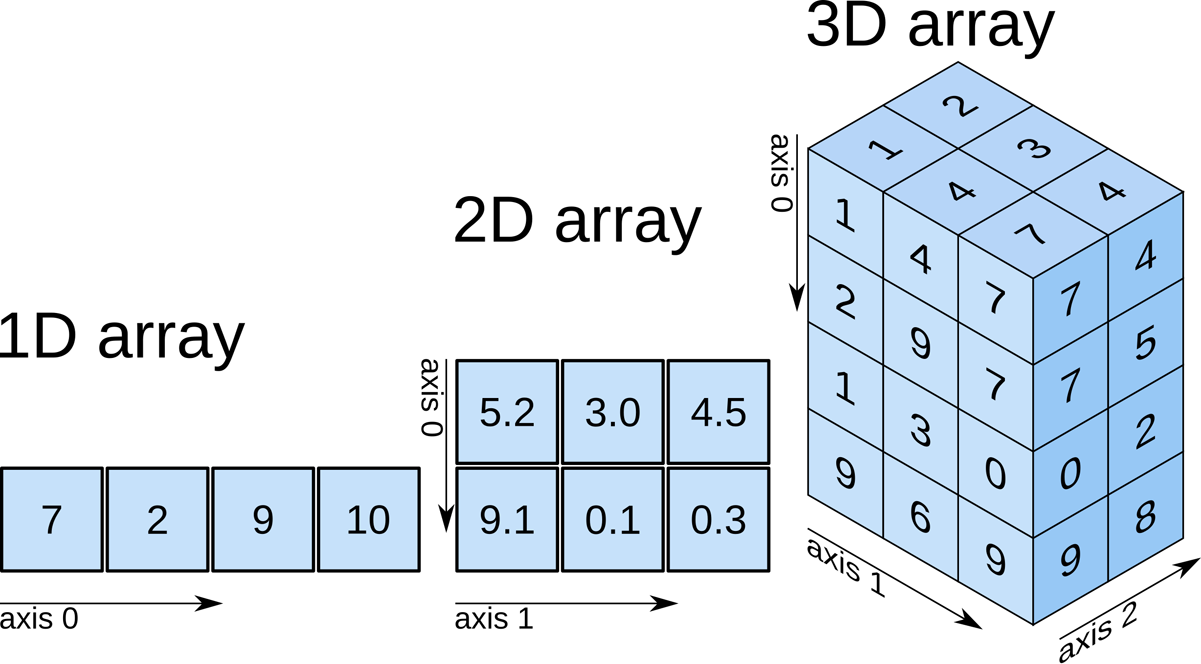
\includegraphics{nda.png}
\end{itemize}

\hypertarget{how-to-create-ndarray}{%
\subsection{How to create ndarray:}\label{how-to-create-ndarray}}

Ndarrays are created using the \texttt{numpy.array} function, which
takes a list or tuple of values as input and returns an ndarray object.

\begin{Shaded}
\begin{Highlighting}[]
\NormalTok{a }\OperatorTok{=}\NormalTok{ np.array([}\DecValTok{1}\NormalTok{,}\DecValTok{2}\NormalTok{,}\DecValTok{3}\NormalTok{]) }\CommentTok{\#1D array}
\NormalTok{b }\OperatorTok{=}\NormalTok{ np.array([(}\FloatTok{1.5}\NormalTok{,}\DecValTok{2}\NormalTok{,}\DecValTok{3}\NormalTok{), (}\DecValTok{4}\NormalTok{,}\DecValTok{5}\NormalTok{,}\DecValTok{6}\NormalTok{)], dtype }\OperatorTok{=} \BuiltInTok{float}\NormalTok{) }\CommentTok{\#2D array}
\NormalTok{c }\OperatorTok{=}\NormalTok{ np.array([[(}\FloatTok{1.5}\NormalTok{,}\DecValTok{2}\NormalTok{,}\DecValTok{3}\NormalTok{), (}\DecValTok{4}\NormalTok{,}\DecValTok{5}\NormalTok{,}\DecValTok{6}\NormalTok{)], [(}\DecValTok{3}\NormalTok{,}\DecValTok{2}\NormalTok{,}\DecValTok{1}\NormalTok{), (}\DecValTok{4}\NormalTok{,}\DecValTok{5}\NormalTok{,}\DecValTok{6}\NormalTok{)]], dtype }\OperatorTok{=} \BuiltInTok{float}\NormalTok{) }\CommentTok{\#3D array}
\end{Highlighting}
\end{Shaded}

\hypertarget{some-important-numpy-array-creation-functions}{%
\subsection{Some important NumPy array creation
functions:}\label{some-important-numpy-array-creation-functions}}
$$
\begin{array}{|l|l|}
  \hline
\text{function}& \text{Description}\\
\hline
\texttt{np.zeros} &\text{Produce an array of all \emph{0s} with the given
shape and data type} \\
\texttt{np.ones} &\text{Produce an array of all \emph{1s} with the given
shape and data type} \\
\texttt{np.arange} &\text{Like the built-in range but returns an ndarray
instead of a list} \\
\texttt{np.linspace} &\text{Create an array of evenly spaced values (number
of samples)} \\
\texttt{np.full} &\text{Produce an array of the given shape and}\\
& \text{data type with all values set to the indicated `fill value';} \\
\texttt{np.eye} or \texttt{np.identity} &\text{Create a square N × N identity}\\
& \text{
matrix (1s on the diagonal and 0s elsewhere)} \\
\texttt{np.random.random} &\text{Create an array with random values} \\
\texttt{np.empty} &\text{Create new arrays by allocating new memory, }\\
& \text{but do
not populate with any values like ones and zeros} \\
\hline
\end{array}
$$
examples:

\begin{Shaded}
\begin{Highlighting}[]
\NormalTok{np.zeros((}\DecValTok{3}\NormalTok{,}\DecValTok{4}\NormalTok{)) }\CommentTok{\#Create an array of zeros}
\NormalTok{np.ones((}\DecValTok{2}\NormalTok{,}\DecValTok{3}\NormalTok{,}\DecValTok{4}\NormalTok{),dtype}\OperatorTok{=}\NormalTok{np.int16) }\CommentTok{\#Create an array of ones}
\NormalTok{np.arange(}\DecValTok{10}\NormalTok{,}\DecValTok{25}\NormalTok{,}\DecValTok{5}\NormalTok{) }\CommentTok{\#Create an array of evenly spaced values (step value)}
\NormalTok{np.linspace(}\DecValTok{0}\NormalTok{,}\DecValTok{2}\NormalTok{,}\DecValTok{9}\NormalTok{) }\CommentTok{\#Create an array of evenly spaced values (number of samples)}
\NormalTok{np.full((}\DecValTok{2}\NormalTok{,}\DecValTok{2}\NormalTok{),}\DecValTok{7}\NormalTok{) }\CommentTok{\#Create a constant array}
\NormalTok{np.eye(}\DecValTok{2}\NormalTok{) }\CommentTok{\#Create a 2X2 identity matrix}
\NormalTok{np.random.random((}\DecValTok{2}\NormalTok{,}\DecValTok{2}\NormalTok{)) }\CommentTok{\#Create an array with random values}
\NormalTok{np.random.randint(}\DecValTok{2}\NormalTok{, size}\OperatorTok{=}\NormalTok{(}\DecValTok{3}\NormalTok{,}\DecValTok{3}\NormalTok{))}
\NormalTok{np.empty((}\DecValTok{3}\NormalTok{,}\DecValTok{2}\NormalTok{)) }\CommentTok{\#Create an empty array}
\end{Highlighting}
\end{Shaded}

\hypertarget{why-not-just-use-python-lists-for-calculations-instead-of-creating-a-new-type-of-array-using-numpy}{%
\subsection{Why not just use Python lists for calculations instead of
creating a new type of array using
numpy?}\label{why-not-just-use-python-lists-for-calculations-instead-of-creating-a-new-type-of-array-using-numpy}}

There are several reasons for this: - Python lists are very general
(also called high-level objects). They can contain any object
\(\Rightarrow\) dynamic typing. They do not support mathematical
operations. - NumPy arrays are statically typed and homogeneous. - The
type of the elements is determined when the array is created
\(\Rightarrow\) no more dynamic typing. - Similarly, the size of the
array is fixed at creation \(\Rightarrow\) optimized memory storage. -
Due to static typing, mathematical functions such as matrix
multiplication and addition can be implemented using a compiled language
(C and Fortran).

Example:

\begin{Shaded}
\begin{Highlighting}[]
\OperatorTok{\%}\NormalTok{timeit [i}\OperatorTok{**}\DecValTok{2} \ControlFlowTok{for}\NormalTok{ i }\KeywordTok{in} \BuiltInTok{range}\NormalTok{(}\DecValTok{1000}\NormalTok{)]}
\NormalTok{a }\OperatorTok{=}\NormalTok{ np.arange(}\DecValTok{1000}\NormalTok{)}
\OperatorTok{\%}\NormalTok{timeit a}\OperatorTok{**}\DecValTok{2}
\end{Highlighting}
\end{Shaded}

\hypertarget{data-types-in-numpy}{%
\subsection{Data types in numpy:}\label{data-types-in-numpy}}

NumPy provides several data types that can be used to create arrays.
$$
\begin{array}{|l|l|l|}
  \hline
Type&Code& Decription\\
\hline
bool &    ? & \text{Boolean (True or False) stored as a byte} \\
int8 &    i1 & \text{Byte (-128 to 127)} \\
int16 &   i2 & \text{Integer (-32768 to 32767)} \\
int32 &   i4 & \text{Integer (-2 ** 31 to 2 ** 31 - 1)} \\
int64 &   i8 & \text{Integer (-2 ** 63 to 2 ** 63 - 1)} \\
uint8 &   u1 & \text{Unsigned integer (0 to 255)} \\
uint16 &  u2 & \text{Unsigned integer (0 to 65535)} \\
uint32 &  u4 & \text{Unsigned integer (0 to 2 ** 32 - 1)} \\
uint64 &  u8 & \text{Unsigned integer (0 to 2 ** 64 - 1)} \\
float16 & f2 & \text{Half precision float} \\
float32 & f4 & \text{Single precision float} \\
float64 & f8 & \text{Double precision float} \\
complex64 & c8 & \text{Complex number, represented by two 32-bit floats} \\
complex128 & c16 & \text{Complex number, represented by two 64-bit floats} \\
string\_& S & \text{Fixed-length ASCII string type (1 byte per character);}\\
&& \text{for example, to create a string data type with length 10, use `S10'} \\
\hline
\end{array}
$$
Example:

\begin{Shaded}
\begin{Highlighting}[]
\NormalTok{a }\OperatorTok{=}\NormalTok{ np.array([}\DecValTok{1}\NormalTok{, }\DecValTok{2}\NormalTok{, }\DecValTok{3}\NormalTok{], dtype}\OperatorTok{=}\NormalTok{?)}
\BuiltInTok{print}\NormalTok{(a)}
\NormalTok{a }\OperatorTok{=}\NormalTok{ np.array([}\DecValTok{1}\NormalTok{, }\DecValTok{2}\NormalTok{, }\DecValTok{3}\NormalTok{], dtype}\OperatorTok{=}\NormalTok{f4)}
\BuiltInTok{print}\NormalTok{(a)}
\end{Highlighting}
\end{Shaded}

\hypertarget{getting-arrays-dimensions-and-data-type-in-numpy}{%
\subsection{Getting arrays dimensions and Data type in
numpy}\label{getting-arrays-dimensions-and-data-type-in-numpy}}

\begin{itemize}
\tightlist
\item
  To get the dimensions of an array, we can use the \texttt{shape}
  attribute. For example, for an array \texttt{a}, we can get its
  dimensions as follows:
\end{itemize}

\begin{Shaded}
\begin{Highlighting}[]
\NormalTok{a }\OperatorTok{=}\NormalTok{ np.array([[}\DecValTok{1}\NormalTok{, }\DecValTok{2}\NormalTok{, }\DecValTok{3}\NormalTok{], [}\DecValTok{4}\NormalTok{, }\DecValTok{5}\NormalTok{, }\DecValTok{6}\NormalTok{]])}
\BuiltInTok{print}\NormalTok{(a.shape)}
\end{Highlighting}
\end{Shaded}

\begin{itemize}
\tightlist
\item
  To get the number of dimensions of an array, we can use the
  \texttt{ndim} attribute. For example:
\end{itemize}

\begin{Shaded}
\begin{Highlighting}[]
\NormalTok{a }\OperatorTok{=}\NormalTok{ np.array([[}\DecValTok{1}\NormalTok{, }\DecValTok{2}\NormalTok{, }\DecValTok{3}\NormalTok{], [}\DecValTok{4}\NormalTok{, }\DecValTok{5}\NormalTok{, }\DecValTok{6}\NormalTok{]])}
\BuiltInTok{print}\NormalTok{(a.ndim)}
\end{Highlighting}
\end{Shaded}

\begin{itemize}
\tightlist
\item
  To get the data type of an array, we can use the \texttt{dtype}
  attribute. For example:
\end{itemize}

\begin{Shaded}
\begin{Highlighting}[]
\NormalTok{a }\OperatorTok{=}\NormalTok{ np.array([}\DecValTok{1}\NormalTok{, }\DecValTok{2}\NormalTok{, }\DecValTok{3}\NormalTok{], dtype}\OperatorTok{=}\NormalTok{np.float32)}
\BuiltInTok{print}\NormalTok{(a.dtype)}
\end{Highlighting}
\end{Shaded}

\begin{itemize}
\tightlist
\item
  We can also explicitly convert the data type of an array using the
  \texttt{astype()} method. For example:
\end{itemize}

\begin{Shaded}
\begin{Highlighting}[]
\NormalTok{a }\OperatorTok{=}\NormalTok{ np.array([}\DecValTok{1}\NormalTok{, }\DecValTok{2}\NormalTok{, }\DecValTok{3}\NormalTok{], dtype}\OperatorTok{=}\NormalTok{np.int32)}
\NormalTok{b }\OperatorTok{=}\NormalTok{ a.astype(np.float32)}
\BuiltInTok{print}\NormalTok{(b.dtype)}
\end{Highlighting}
\end{Shaded}

\hypertarget{array-mathematics-in-numpy}{%
\subsection{Array mathematics in
numpy:}\label{array-mathematics-in-numpy}}

\hypertarget{arithmetic-operations}{%
\subsubsection{Arithmetic Operations}\label{arithmetic-operations}}

\hypertarget{subtraction-addition-division-multiplication-item-per-item}{%
\paragraph{Subtraction, Addition, Division, Multiplication (item per
item):}\label{subtraction-addition-division-multiplication-item-per-item}}

NumPy provides element-wise arithmetic operations for arrays. You can
perform addition, subtraction, multiplication, and division on arrays by
simply using the appropriate operator \texttt{(+,\ -,\ *,\ /)} between
them. The operations are performed on each corresponding element of the
arrays. For example:

\begin{Shaded}
\begin{Highlighting}[]

\NormalTok{a }\OperatorTok{=}\NormalTok{ np.array([}\DecValTok{1}\NormalTok{, }\DecValTok{2}\NormalTok{, }\DecValTok{3}\NormalTok{])}
\NormalTok{b }\OperatorTok{=}\NormalTok{ np.array([}\DecValTok{4}\NormalTok{, }\DecValTok{5}\NormalTok{, }\DecValTok{6}\NormalTok{])}

\CommentTok{\# Addition}
\NormalTok{c }\OperatorTok{=}\NormalTok{ a }\OperatorTok{+}\NormalTok{ b}
\BuiltInTok{print}\NormalTok{(c)  }\CommentTok{\# Output: [5 7 9]}

\CommentTok{\# Subtraction}
\NormalTok{d }\OperatorTok{=}\NormalTok{ a }\OperatorTok{{-}}\NormalTok{ b}
\BuiltInTok{print}\NormalTok{(d)  }\CommentTok{\# Output: [{-}3 {-}3 {-}3]}

\CommentTok{\# Multiplication}
\NormalTok{e }\OperatorTok{=}\NormalTok{ a }\OperatorTok{*}\NormalTok{ b}
\BuiltInTok{print}\NormalTok{(e)  }\CommentTok{\# Output: [ 4 10 18]}

\CommentTok{\# Division}
\NormalTok{f }\OperatorTok{=}\NormalTok{ a }\OperatorTok{/}\NormalTok{ b}
\BuiltInTok{print}\NormalTok{(f)  }\CommentTok{\# Output: [0.25 0.4  0.5 ]}
\end{Highlighting}
\end{Shaded}

\hypertarget{element-wise-mathematical-functions}{%
\paragraph{element-wise mathematical
functions:}\label{element-wise-mathematical-functions}}

NumPy provides several mathematical functions that operate element-wise
on arrays. For example,

\begin{Shaded}
\begin{Highlighting}[]
\ImportTok{import}\NormalTok{ numpy }\ImportTok{as}\NormalTok{ np}

\NormalTok{a }\OperatorTok{=}\NormalTok{ np.array([}\DecValTok{1}\NormalTok{, }\DecValTok{4}\NormalTok{, }\DecValTok{9}\NormalTok{])}

\CommentTok{\# Square root}
\NormalTok{b }\OperatorTok{=}\NormalTok{ np.sqrt(a)}
\BuiltInTok{print}\NormalTok{(b)  }\CommentTok{\# Output: [1. 2. 3.]}

\CommentTok{\# Sine}
\NormalTok{c }\OperatorTok{=}\NormalTok{ np.sin(a)}
\BuiltInTok{print}\NormalTok{(c)  }\CommentTok{\# Output: [ 0.84147098 {-}0.7568025   0.41211849]}

\CommentTok{\# Cosine}
\NormalTok{d }\OperatorTok{=}\NormalTok{ np.cos(a)}
\BuiltInTok{print}\NormalTok{(d)  }\CommentTok{\# Output: [ 0.54030231 {-}0.65364362 {-}0.91113026]}
\end{Highlighting}
\end{Shaded}

\hypertarget{comparison}{%
\subsubsection{Comparison}\label{comparison}}

In NumPy, we can compare arrays element-wise using comparison operators
such as \texttt{==,\ !=,\ \textless{},\ \textgreater{},\ \textless{}=,}
and \texttt{\textgreater{}=}. When performing element-wise comparisons,
the result is a boolean array of the same shape as the original arrays.
For example:

\begin{Shaded}
\begin{Highlighting}[]
\NormalTok{a }\OperatorTok{=}\NormalTok{ np.array([}\DecValTok{1}\NormalTok{, }\DecValTok{2}\NormalTok{, }\DecValTok{3}\NormalTok{])}
\NormalTok{b }\OperatorTok{=}\NormalTok{ np.array([}\DecValTok{1}\NormalTok{, }\DecValTok{2}\NormalTok{, }\DecValTok{4}\NormalTok{])}

\BuiltInTok{print}\NormalTok{(a }\OperatorTok{==}\NormalTok{ b)  }\CommentTok{\# [ True  True False]}
\BuiltInTok{print}\NormalTok{(a }\OperatorTok{!=}\NormalTok{ b)  }\CommentTok{\# [False False  True]}
\BuiltInTok{print}\NormalTok{(a }\OperatorTok{\textless{}}\NormalTok{ b)   }\CommentTok{\# [False False  True]}
\BuiltInTok{print}\NormalTok{(a }\OperatorTok{\textgreater{}}\NormalTok{ b)   }\CommentTok{\# [False False False]}
\BuiltInTok{print}\NormalTok{(a }\OperatorTok{\textless{}=}\NormalTok{ b)  }\CommentTok{\# [ True  True  True]}
\BuiltInTok{print}\NormalTok{(a }\OperatorTok{\textgreater{}=}\NormalTok{ b)  }\CommentTok{\# [ True  True False]}
\end{Highlighting}
\end{Shaded}

we can also perform element-wise comparisons between a scalar value and
an array:

\begin{Shaded}
\begin{Highlighting}[]
\NormalTok{a }\OperatorTok{=}\NormalTok{ np.array([}\DecValTok{1}\NormalTok{, }\DecValTok{2}\NormalTok{, }\DecValTok{3}\NormalTok{])}
\NormalTok{b }\OperatorTok{=} \DecValTok{2}

\BuiltInTok{print}\NormalTok{(a }\OperatorTok{==}\NormalTok{ b)  }\CommentTok{\# [False  True False]}
\BuiltInTok{print}\NormalTok{(a }\OperatorTok{!=}\NormalTok{ b)  }\CommentTok{\# [ True False  True]}
\BuiltInTok{print}\NormalTok{(a }\OperatorTok{\textless{}}\NormalTok{ b)   }\CommentTok{\# [ True False False]}
\BuiltInTok{print}\NormalTok{(a }\OperatorTok{\textgreater{}}\NormalTok{ b)   }\CommentTok{\# [False False  True]}
\BuiltInTok{print}\NormalTok{(a }\OperatorTok{\textless{}=}\NormalTok{ b)  }\CommentTok{\# [ True  True False]}
\BuiltInTok{print}\NormalTok{(a }\OperatorTok{\textgreater{}=}\NormalTok{ b)  }\CommentTok{\# [False  True  True]}
\end{Highlighting}
\end{Shaded}

\hypertarget{any-all-and-sum-with-condition}{%
\paragraph{any(), all(), and sum() with
condition:}\label{any-all-and-sum-with-condition}}

\begin{itemize}
\item
  \texttt{all()} returns True if all the elements in the input array
  evaluate to True. Otherwise, it returns False.
\item
  \texttt{any()} returns True if any of the elements in the input array
  evaluate to True. Otherwise, it returns False.
\end{itemize}

Here are some examples:

\begin{Shaded}
\begin{Highlighting}[]
\ImportTok{import}\NormalTok{ numpy }\ImportTok{as}\NormalTok{ np}

\NormalTok{a }\OperatorTok{=}\NormalTok{ np.array([}\DecValTok{1}\NormalTok{, }\DecValTok{2}\NormalTok{, }\DecValTok{3}\NormalTok{, }\DecValTok{4}\NormalTok{])}
\NormalTok{b }\OperatorTok{=}\NormalTok{ np.array([}\DecValTok{0}\NormalTok{, }\DecValTok{2}\NormalTok{, }\DecValTok{4}\NormalTok{, }\DecValTok{6}\NormalTok{])}
\NormalTok{c }\OperatorTok{=}\NormalTok{ np.array([}\OperatorTok{{-}}\DecValTok{1}\NormalTok{, }\DecValTok{2}\NormalTok{, }\OperatorTok{{-}}\DecValTok{3}\NormalTok{, }\DecValTok{4}\NormalTok{])}

\CommentTok{\# using all() method}
\BuiltInTok{print}\NormalTok{(np.}\BuiltInTok{all}\NormalTok{(a }\OperatorTok{\textgreater{}} \DecValTok{0}\NormalTok{))   }\CommentTok{\# True}
\BuiltInTok{print}\NormalTok{(np.}\BuiltInTok{all}\NormalTok{(b }\OperatorTok{\textgreater{}} \DecValTok{0}\NormalTok{))   }\CommentTok{\# False}
\BuiltInTok{print}\NormalTok{(np.}\BuiltInTok{all}\NormalTok{(c }\OperatorTok{\textgreater{}} \DecValTok{0}\NormalTok{))   }\CommentTok{\# False}

\CommentTok{\# using any() method}
\BuiltInTok{print}\NormalTok{(np.}\BuiltInTok{any}\NormalTok{(a }\OperatorTok{==} \DecValTok{2}\NormalTok{))  }\CommentTok{\# True}
\BuiltInTok{print}\NormalTok{(np.}\BuiltInTok{any}\NormalTok{(b }\OperatorTok{==} \DecValTok{1}\NormalTok{))  }\CommentTok{\# False}
\BuiltInTok{print}\NormalTok{(np.}\BuiltInTok{any}\NormalTok{(c }\OperatorTok{==} \OperatorTok{{-}}\DecValTok{3}\NormalTok{)) }\CommentTok{\# True}
\end{Highlighting}
\end{Shaded}

\begin{itemize}
\tightlist
\item
  In NumPy, we can perform sum with condition using the
  \texttt{np.sum()} function with a boolean mask as input. The boolean
  mask is created using a comparison operator
  (\texttt{\textgreater{},\ \textless{},\ ==,} etc.) on an array, which
  creates a boolean array of the same shape with True where the
  condition is met and False where it is not.
\end{itemize}

\begin{Shaded}
\begin{Highlighting}[]
\ImportTok{import}\NormalTok{ numpy }\ImportTok{as}\NormalTok{ np}

\CommentTok{\# Create an array}
\NormalTok{arr }\OperatorTok{=}\NormalTok{ np.array([[}\DecValTok{1}\NormalTok{, }\DecValTok{2}\NormalTok{, }\DecValTok{3}\NormalTok{], [}\DecValTok{4}\NormalTok{, }\DecValTok{5}\NormalTok{, }\DecValTok{6}\NormalTok{], [}\DecValTok{7}\NormalTok{, }\DecValTok{8}\NormalTok{, }\DecValTok{9}\NormalTok{]])}

\CommentTok{\# Sum all elements that are greater than 5}
\NormalTok{sum\_greater\_than\_5 }\OperatorTok{=}\NormalTok{ np.}\BuiltInTok{sum}\NormalTok{(arr[arr }\OperatorTok{\textgreater{}} \DecValTok{5}\NormalTok{])}

\BuiltInTok{print}\NormalTok{(sum\_greater\_than\_5) }\CommentTok{\# Output: 30}
\end{Highlighting}
\end{Shaded}

\hypertarget{arrays-statistics-functions}{%
\subsubsection{Arrays statistics
functions:}\label{arrays-statistics-functions}}

NumPy provides many built-in statistical functions that can be used to
perform various statistical operations on arrays. Here are some of the
commonly used statistical functions in NumPy:
$$
\begin{array}{|l|l|}
  \hline
function &  Description\\
\hline
np.mean() &\text{ Calculates the arithmetic mean of an array along a specified
axis.} \\
np.median() &\text{ Computes the median of an array along a specified axis.} \\
np.std() &\text{ Computes the standard deviation of an array along a specified
axis.} \\
np.var() &\text{ Computes the variance of an array along a specified axis.} \\
np.min() &\text{ Computes the minimum value of an array along a specified
axis.} \\
np.max() &\text{ Computes the maximum value of an array along a specified
axis.} \\
np.argmin() &\text{ Return the index of the minimum value} \\
np.argmax() &\text{ Return the index of the maximum value} \\
np.sum() &\text{ Computes the sum of all the elements in an array along a
specified axis.} \\
np.prod() &\text{ Computes the product of all the elements in an array along a
specified axis.} \\
np.cumsum() &\text{ Computes the cumulative sum of the elements in an array
along a specified axis.} \\
\hline
\end{array}
$$
Here's an example of how to use some of these functions:

\begin{Shaded}
\begin{Highlighting}[]
\ImportTok{import}\NormalTok{ numpy }\ImportTok{as}\NormalTok{ np}

\NormalTok{a }\OperatorTok{=}\NormalTok{ np.array([[}\DecValTok{1}\NormalTok{, }\DecValTok{2}\NormalTok{, }\DecValTok{3}\NormalTok{], [}\DecValTok{4}\NormalTok{, }\DecValTok{5}\NormalTok{, }\DecValTok{6}\NormalTok{], [}\DecValTok{7}\NormalTok{, }\DecValTok{8}\NormalTok{, }\DecValTok{9}\NormalTok{]])}

\BuiltInTok{print}\NormalTok{(np.mean(a))          }\CommentTok{\# 5.0}
\BuiltInTok{print}\NormalTok{(np.median(a))        }\CommentTok{\# 5.0}
\BuiltInTok{print}\NormalTok{(np.std(a))           }\CommentTok{\# 2.581988897471611}
\BuiltInTok{print}\NormalTok{(np.var(a))           }\CommentTok{\# 6.666666666666667}
\BuiltInTok{print}\NormalTok{(np.}\BuiltInTok{min}\NormalTok{(a,axis}\OperatorTok{=}\DecValTok{1}\NormalTok{))     }\CommentTok{\# [1 4 7]}
\BuiltInTok{print}\NormalTok{(np.}\BuiltInTok{max}\NormalTok{(a))           }\CommentTok{\# 9}
\BuiltInTok{print}\NormalTok{(np.}\BuiltInTok{sum}\NormalTok{(a))           }\CommentTok{\# 45}
\BuiltInTok{print}\NormalTok{(np.prod(a))          }\CommentTok{\# 362880}
\BuiltInTok{print}\NormalTok{(np.cumsum(a))        }\CommentTok{\# [ 1  3  6 10 15 21 28 36 45]}
\end{Highlighting}
\end{Shaded}

\hypertarget{arrays-algebraic-and-form-operations}{%
\subsubsection{Arrays algebraic and form
operations:}\label{arrays-algebraic-and-form-operations}}

\hypertarget{dot-product}{%
\paragraph{Dot product}\label{dot-product}}

The \texttt{dot()} function in NumPy performs matrix multiplication or
dot product of two arrays.

\begin{Shaded}
\begin{Highlighting}[]
\NormalTok{A }\OperatorTok{=}\NormalTok{ np.array([[}\DecValTok{1}\NormalTok{, }\DecValTok{2}\NormalTok{], [}\DecValTok{3}\NormalTok{, }\DecValTok{4}\NormalTok{], [}\DecValTok{5}\NormalTok{, }\DecValTok{6}\NormalTok{]])}
\NormalTok{B }\OperatorTok{=}\NormalTok{ np.array([[}\DecValTok{7}\NormalTok{, }\DecValTok{8}\NormalTok{], [}\DecValTok{9}\NormalTok{, }\DecValTok{10}\NormalTok{]])}

\CommentTok{\# Matrix multiplication of A and B}
\NormalTok{C }\OperatorTok{=}\NormalTok{ np.dot(A, B )}\CommentTok{\# or C = A @ B}
\BuiltInTok{print}\NormalTok{(C)}
\end{Highlighting}
\end{Shaded}

\hypertarget{transposition}{%
\paragraph{Transposition}\label{transposition}}

The \texttt{transpose()} function can be called on a NumPy array to
create a new array with the rows and columns flipped. For example, the
following code creates a 2D array arr and then transposes it using the
\texttt{transpose()} function:

\begin{Shaded}
\begin{Highlighting}[]
\NormalTok{arr }\OperatorTok{=}\NormalTok{ np.array([[}\DecValTok{1}\NormalTok{, }\DecValTok{2}\NormalTok{], [}\DecValTok{3}\NormalTok{, }\DecValTok{4}\NormalTok{]])}
\NormalTok{transposed\_arr }\OperatorTok{=}\NormalTok{ np.transpose(arr)}
\BuiltInTok{print}\NormalTok{(transposed\_arr)}
\end{Highlighting}
\end{Shaded}

Alternatively, the \texttt{T} attribute can be used to transpose an
array. For example:

\begin{Shaded}
\begin{Highlighting}[]
\NormalTok{arr }\OperatorTok{=}\NormalTok{ np.array([[}\DecValTok{1}\NormalTok{, }\DecValTok{2}\NormalTok{], [}\DecValTok{3}\NormalTok{, }\DecValTok{4}\NormalTok{]])}
\NormalTok{transposed\_arr }\OperatorTok{=}\NormalTok{ arr.T}
\BuiltInTok{print}\NormalTok{(transposed\_arr)}
\end{Highlighting}
\end{Shaded}

\hypertarget{reshaping}{%
\paragraph{Reshaping:}\label{reshaping}}

Changing the shape of an array while maintaining the same number of
elements.

\begin{Shaded}
\begin{Highlighting}[]
\ImportTok{import}\NormalTok{ numpy }\ImportTok{as}\NormalTok{ np}
\NormalTok{a }\OperatorTok{=}\NormalTok{ np.array([[}\DecValTok{1}\NormalTok{, }\DecValTok{2}\NormalTok{], [}\DecValTok{3}\NormalTok{, }\DecValTok{4}\NormalTok{], [}\DecValTok{5}\NormalTok{, }\DecValTok{6}\NormalTok{]])}
\BuiltInTok{print}\NormalTok{(}\StringTok{"Original array:}\CharTok{\textbackslash{}n}\StringTok{"}\NormalTok{, a)}
\CommentTok{\# Output: }
\CommentTok{\# Original array:}
\CommentTok{\#  [[1 2]}
\CommentTok{\#   [3 4]}
\CommentTok{\#   [5 6]]}

\NormalTok{b }\OperatorTok{=}\NormalTok{ a.reshape((}\DecValTok{2}\NormalTok{, }\DecValTok{3}\NormalTok{))}
\BuiltInTok{print}\NormalTok{(}\StringTok{"Reshaped array:}\CharTok{\textbackslash{}n}\StringTok{"}\NormalTok{, b)}
\CommentTok{\# Output: }
\CommentTok{\# Reshaped array:}
\CommentTok{\#  [[1 2 3]}
\CommentTok{\#   [4 5 6]]}
\end{Highlighting}
\end{Shaded}

\hypertarget{broadcasting}{%
\paragraph{Broadcasting:}\label{broadcasting}}

Performing operations on arrays with different shapes and sizes.

\begin{Shaded}
\begin{Highlighting}[]
\ImportTok{import}\NormalTok{ numpy }\ImportTok{as}\NormalTok{ np}
\NormalTok{a }\OperatorTok{=}\NormalTok{ np.array([}\DecValTok{1}\NormalTok{, }\DecValTok{2}\NormalTok{, }\DecValTok{3}\NormalTok{])}
\NormalTok{b }\OperatorTok{=}\NormalTok{ np.array([[}\DecValTok{4}\NormalTok{], [}\DecValTok{5}\NormalTok{], [}\DecValTok{6}\NormalTok{]])}
\NormalTok{c }\OperatorTok{=}\NormalTok{ a }\OperatorTok{+}\NormalTok{ b}
\BuiltInTok{print}\NormalTok{(}\StringTok{"Result array:}\CharTok{\textbackslash{}n}\StringTok{"}\NormalTok{, c)}
\CommentTok{\# Output:}
\CommentTok{\# Result array:}
\CommentTok{\#  [[5 6 7]}
\CommentTok{\#   [6 7 8]}
\CommentTok{\#   [7 8 9]]}
\end{Highlighting}
\end{Shaded}

\hypertarget{concatenation}{%
\paragraph{Concatenation:}\label{concatenation}}

Joining two or more arrays along a specified axis.

\begin{Shaded}
\begin{Highlighting}[]
\ImportTok{import}\NormalTok{ numpy }\ImportTok{as}\NormalTok{ np}
\NormalTok{a }\OperatorTok{=}\NormalTok{ np.array([[}\DecValTok{1}\NormalTok{, }\DecValTok{2}\NormalTok{], [}\DecValTok{3}\NormalTok{, }\DecValTok{4}\NormalTok{]])}
\NormalTok{b }\OperatorTok{=}\NormalTok{ np.array([[}\DecValTok{5}\NormalTok{, }\DecValTok{6}\NormalTok{]])}
\NormalTok{c }\OperatorTok{=}\NormalTok{ np.concatenate((a, b), axis}\OperatorTok{=}\DecValTok{0}\NormalTok{)}
\BuiltInTok{print}\NormalTok{(}\StringTok{"Concatenated array:}\CharTok{\textbackslash{}n}\StringTok{"}\NormalTok{, c)}
\CommentTok{\# Output:}
\CommentTok{\# Concatenated array:}
\CommentTok{\#  [[1 2]}
\CommentTok{\#   [3 4]}
\CommentTok{\#   [5 6]]}
\end{Highlighting}
\end{Shaded}

\hypertarget{stacking}{%
\paragraph{Stacking:}\label{stacking}}

Joining two or more arrays along a new axis.

\begin{Shaded}
\begin{Highlighting}[]
\ImportTok{import}\NormalTok{ numpy }\ImportTok{as}\NormalTok{ np}
\NormalTok{a }\OperatorTok{=}\NormalTok{ np.array([}\DecValTok{1}\NormalTok{, }\DecValTok{2}\NormalTok{, }\DecValTok{3}\NormalTok{])}
\NormalTok{b }\OperatorTok{=}\NormalTok{ np.array([}\DecValTok{4}\NormalTok{, }\DecValTok{5}\NormalTok{, }\DecValTok{6}\NormalTok{])}
\NormalTok{c }\OperatorTok{=}\NormalTok{ np.stack((a, b), axis}\OperatorTok{=}\DecValTok{0}\NormalTok{)}
\BuiltInTok{print}\NormalTok{(}\StringTok{"Stacked array:}\CharTok{\textbackslash{}n}\StringTok{"}\NormalTok{, c)}
\CommentTok{\# Output:}
\CommentTok{\# Stacked array:}
\CommentTok{\#  [[1 2 3]}
\CommentTok{\#   [4 5 6]]}
\end{Highlighting}
\end{Shaded}

\hypertarget{splitting}{%
\subsubsection{Splitting:}\label{splitting}}

Splitting an array into smaller arrays along a specified axis.

\begin{Shaded}
\begin{Highlighting}[]
\ImportTok{import}\NormalTok{ numpy }\ImportTok{as}\NormalTok{ np}
\NormalTok{a }\OperatorTok{=}\NormalTok{ np.array([[}\DecValTok{1}\NormalTok{, }\DecValTok{2}\NormalTok{, }\DecValTok{3}\NormalTok{], [}\DecValTok{4}\NormalTok{, }\DecValTok{5}\NormalTok{, }\DecValTok{6}\NormalTok{], [}\DecValTok{7}\NormalTok{, }\DecValTok{8}\NormalTok{, }\DecValTok{9}\NormalTok{], [}\DecValTok{10}\NormalTok{, }\DecValTok{11}\NormalTok{, }\DecValTok{12}\NormalTok{]])}
\NormalTok{b, c }\OperatorTok{=}\NormalTok{ np.split(a, }\DecValTok{2}\NormalTok{, axis}\OperatorTok{=}\DecValTok{0}\NormalTok{)}
\BuiltInTok{print}\NormalTok{(}\StringTok{"First split array:}\CharTok{\textbackslash{}n}\StringTok{"}\NormalTok{, b)}
\BuiltInTok{print}\NormalTok{(}\StringTok{"Second split array:}\CharTok{\textbackslash{}n}\StringTok{"}\NormalTok{, c)}
\CommentTok{\# Output:}
\CommentTok{\# First split array:}
\CommentTok{\#  [[1 2 3]}
\CommentTok{\#   [4 5 6]]}
\CommentTok{\# Second split array:}
\CommentTok{\#  [[ 7  8  9]}
\CommentTok{\#   [10 11 12]]}
\end{Highlighting}
\end{Shaded}

\hypertarget{flattened-array}{%
\subsubsection{flattened array}\label{flattened-array}}

\texttt{ravel()} is a function in NumPy that returns a flattened array.
It means that it returns a 1-dimensional array that contains all the
elements of the input array. The returned array is always a copy of the
original array, so modifying it does not affect the original array.

Here is an example of how to use \texttt{ravel()}:

\begin{Shaded}
\begin{Highlighting}[]
\ImportTok{import}\NormalTok{ numpy }\ImportTok{as}\NormalTok{ np}

\CommentTok{\# Create a 2{-}dimensional array}
\NormalTok{arr }\OperatorTok{=}\NormalTok{ np.array([[}\DecValTok{1}\NormalTok{, }\DecValTok{2}\NormalTok{], [}\DecValTok{3}\NormalTok{, }\DecValTok{4}\NormalTok{]])}

\CommentTok{\# Flatten the array using ravel()}
\NormalTok{flat\_arr }\OperatorTok{=}\NormalTok{ arr.ravel()}

\CommentTok{\# Print the original and flattened arrays}
\BuiltInTok{print}\NormalTok{(}\StringTok{"Original array:}\CharTok{\textbackslash{}n}\StringTok{"}\NormalTok{, arr)}
\BuiltInTok{print}\NormalTok{(}\StringTok{"Flattened array:}\CharTok{\textbackslash{}n}\StringTok{"}\NormalTok{, flat\_arr)}
\end{Highlighting}
\end{Shaded}

\hypertarget{copying-arrays}{%
\subsection{Copying Arrays}\label{copying-arrays}}

In NumPy, arrays can be copied in different ways, depending on the
desired behavior. Here are some ways to copy arrays in NumPy:

1- \textbf{Shallow copy}: In this type of copy, a new array object is
created, but the data is not copied. Instead, a reference to the
original data is used. Shallow copy can be made using the
\texttt{view()} method.

2- \textbf{Deep copy}: In this type of copy, a completely new array and
data are created. Deep copy can be made using the \texttt{copy()}
method. Example:

\begin{Shaded}
\begin{Highlighting}[]
\ImportTok{import}\NormalTok{ numpy }\ImportTok{as}\NormalTok{ np}

\NormalTok{arr1 }\OperatorTok{=}\NormalTok{ np.array([}\DecValTok{1}\NormalTok{, }\DecValTok{2}\NormalTok{, }\DecValTok{3}\NormalTok{])}
\NormalTok{arr2 }\OperatorTok{=}\NormalTok{ arr1.view()}

\BuiltInTok{print}\NormalTok{(arr1)}
\BuiltInTok{print}\NormalTok{(arr2)}

\NormalTok{arr2[}\DecValTok{0}\NormalTok{] }\OperatorTok{=} \DecValTok{0}
\BuiltInTok{print}\NormalTok{(}\StringTok{"Shallow copy"}\NormalTok{)}
\BuiltInTok{print}\NormalTok{(arr1)}
\BuiltInTok{print}\NormalTok{(arr2)}

\NormalTok{arr2}\OperatorTok{=}\NormalTok{arr1.copy()}
\NormalTok{arr2[}\DecValTok{2}\NormalTok{] }\OperatorTok{=} \DecValTok{4}
\BuiltInTok{print}\NormalTok{(}\StringTok{"Deep copy"}\NormalTok{)}
\BuiltInTok{print}\NormalTok{(arr1)}
\BuiltInTok{print}\NormalTok{(arr2)}
\end{Highlighting}
\end{Shaded}

\hypertarget{sorting-arrays}{%
\subsection{Sorting Arrays}\label{sorting-arrays}}

Sorting an array in numpy can be done using the \texttt{sort()}
function. By default, it sorts the array in ascending order.

Here is an example:

\begin{Shaded}
\begin{Highlighting}[]
\ImportTok{import}\NormalTok{ numpy }\ImportTok{as}\NormalTok{ np}

\NormalTok{arr }\OperatorTok{=}\NormalTok{ np.array([}\DecValTok{3}\NormalTok{, }\DecValTok{2}\NormalTok{, }\DecValTok{1}\NormalTok{, }\DecValTok{4}\NormalTok{, }\DecValTok{5}\NormalTok{])}
\NormalTok{arr.sort()}

\BuiltInTok{print}\NormalTok{(arr)}
\CommentTok{\#output}
\CommentTok{\#[1 2 3 4 5]}
\end{Highlighting}
\end{Shaded}

If you want to sort a two-dimensional array, you can use the
\texttt{sort()} function with the axis parameter. By default, it sorts
each row independently.

Here is an example:

\begin{Shaded}
\begin{Highlighting}[]
\ImportTok{import}\NormalTok{ numpy }\ImportTok{as}\NormalTok{ np}

\NormalTok{arr }\OperatorTok{=}\NormalTok{ np.array([[}\DecValTok{3}\NormalTok{, }\DecValTok{2}\NormalTok{, }\DecValTok{1}\NormalTok{],}
\NormalTok{                [}\DecValTok{6}\NormalTok{, }\DecValTok{5}\NormalTok{, }\DecValTok{4}\NormalTok{],}
\NormalTok{                [}\DecValTok{9}\NormalTok{, }\DecValTok{8}\NormalTok{, }\DecValTok{7}\NormalTok{]])}

\NormalTok{arr.sort(axis}\OperatorTok{=}\DecValTok{1}\NormalTok{)}
\CommentTok{\#output}
\CommentTok{\#[[1 2 3]}
\CommentTok{\# [4 5 6]}
\CommentTok{\# [7 8 9]]}
\BuiltInTok{print}\NormalTok{(arr)}
\end{Highlighting}
\end{Shaded}




    % Add a bibliography block to the postdoc
    
    
    
\end{document}
